% ==============================================================================
% Fichier : 03_demarche.tex
% Description : Démarche Générale d'Audit des Systèmes d'Information
% ==============================================================================

\chapter{Démarche Générale d'Audit des Systèmes d'Information}%
\label{chap:03_demarche}

Ce chapitre détaille le processus complet d'une mission d'audit des SI, de sa commande
à la remise du rapport et au suivi des recommandations. L'audit des SI peut constituer
un sous-domaine d'un audit généraliste (organisation, processus, régularité) ou être
l'objet principal de la mission (application, projet, sécurité, conformité légale).
Dans les deux cas, la démarche s'articule en quatre phases séquentielles dont le poids
relatif, sur la base de l'expérience de terrain, suit la répartition indicative suivante~:

\begin{table}[h!]
\centering
\small
\renewcommand{\arraystretch}{1.4}
\begin{tabular}{|l|c|l|}
    \hline
    \rowcolor{blue!10}
    \textbf{Phase} & \textbf{Part du temps} & \textbf{Livrable principal} \\ \hline
    Travaux préparatoires & 15\,\% & Lettre de mission, TDR, ordres de mission \\ \hline
    Planification & 35\,\% & Rapport d'orientation \\ \hline
    Exécution & 30\,\% & Papiers de travail, projets d'observation \\ \hline
    Communication des résultats & 15\,\% & Rapport final \\ \hline
    Imprévus & 5\,\% & — \\ \hline
\end{tabular}
\caption{Répartition indicative du temps d'une mission d'audit des SI}
\end{table}

% ==============================================================================
\section{Le Cadre Normatif et Déontologique de la Mission}
\label{sec:cadre-normatif}
% ==============================================================================

Avant d'agir, l'auditeur doit connaître les règles du jeu~: celles qui encadrent
son comportement et celles qui fondent son mandat.

% ------------------------------------------------------------------------------
\subsection{La Référence Absolue~: ISO~19011}
\label{subsec:iso19011}
% ------------------------------------------------------------------------------

\begin{boxdef}
\textbf{ISO~19011 (Lignes directrices pour l'audit des systèmes de management)~:}
Norme universelle qui définit \emph{comment} auditer, indépendamment du domaine
audité. Elle pose six principes éthiques qui gouvernent le comportement de l'auditeur
avant, pendant et après la mission.
\end{boxdef}

\subsubsection{Les Six Principes de l'Audit}

\begin{table}[h!]
\centering
\small
\begin{tabular}{p{3cm}p{5cm}p{5cm}}
    \toprule
    \textbf{Principe} & \textbf{Définition} & \textbf{Application Lizbiz's} \\
    \midrule
    \textbf{Intégrité} & Être honnête, responsable et éthique. &
        L'auditeur ne cache pas les problèmes détectés, même s'ils sont
        gênants pour la direction. \\
    \midrule
    \textbf{Présentation équitable} & Rendre compte avec exactitude et vérité. &
        Le rapport reflète fidèlement les preuves~; on ne grossit pas
        les risques mineurs. \\
    \midrule
    \textbf{Devoir de vigilance} & Faire preuve de jugement professionnel. &
        L'auditeur évite de perturber la production (ex~: tests de charge
        en heure de pointe). \\
    \midrule
    \textbf{Confidentialité} & Protéger l'information sensible. &
        L'auditeur ne divulgue pas les failles de sécurité de Lizbiz's
        à l'extérieur. \\
    \midrule
    \textbf{Indépendance} & Être impartial et sans conflit d'intérêt. &
        L'auditeur ne réalise pas l'audit de l'application qu'il a
        lui-même développée. \\
    \midrule
    \textbf{Approche fondée sur la preuve} & Baser les conclusions sur
        des faits vérifiables. &
        \og{}Le serveur n'est pas à jour\fg{} est constaté par capture
        d'écran, pas par ouï-dire. \\
    \bottomrule
\end{tabular}
\caption{Les 6~principes de l'audit selon ISO~19011}
\end{table}

% ------------------------------------------------------------------------------
\subsection{Le Référentiel IFACI~: La Charte d'Audit}
\label{subsec:charte-audit}
% ------------------------------------------------------------------------------

Pour l'audit interne, le référentiel de l'\textbf{IFACI} (Institut Français de
l'Audit et du Contrôle Internes) impose l'existence d'une \textbf{Charte d'Audit}.

\begin{boxdef}
\textbf{Charte d'Audit~:} Document officiel qui définit le mandat de l'audit,
son positionnement hiérarchique, ses pouvoirs d'investigation et l'étendue de
ses compétences. C'est le titre de propriété de l'auditeur~: sans elle, il est
désarmé face à tout refus de coopération.
\end{boxdef}

\begin{boxlizbiz}
\textbf{Cas Lizbiz's~:}
Si le DSI refuse l'accès aux journaux d'exploitation, l'auditeur invoque la
\textbf{Charte d'Audit} signée par le PDG, qui stipule que \og{}l'audit a accès
illimité à tous les documents nécessaires à l'exercice de sa mission\fg{}.
Sans cette charte, le refus ne peut être formellement contesté.
\end{boxlizbiz}

% ==============================================================================
\section{Champs d'Application}
\label{sec:champs-application}
% ==============================================================================

L'audit des SI n'est pas monolithique~: son objet varie selon la commande
du mandant. Quatre configurations sont courantes.

\subsection{Audit d'une Organisation}

Toute organisation dépend aujourd'hui de son SI pour sa performance opérationnelle.
L'audit d'une organisation doit donc nécessairement inclure un audit de sa relation
à l'informatique~: comment définit-elle ses besoins fonctionnels, comment alloue-t-elle
ses ressources pour les satisfaire, s'est-elle organisée pour disposer d'un SI aligné,
réactif, sûr et efficient~?

\subsection{Audit de Processus}

Dans une organisation pilotée par les processus, les outils informatiques en
automatisent tout ou partie. L'audit d'un processus doit inclure l'examen des données
manipulées, des applications qui le servent et des infrastructures de traitement et de
communication qu'il utilise.

\subsection{Audit de Régularité}

Vérifier la régularité d'une situation implique d'auditer les ressources informatiques
qui y contribuent. L'auditeur évalue à la fois la valeur de la contribution de
l'informatique à la régularité des opérations auditées \emph{et} la régularité des
activités informatiques elles-mêmes.

\subsection{Audit des Fonctions Externalisées}

L'externalisation d'une fonction implique presque toujours une interconnexion des SI
et une délégation de responsabilités sur des données appartenant au patrimoine de
l'organisation. La dimension informatique de l'externalisation est au cœur de sa
réversibilité~; elle peut en être la cause d'irréversibilité. L'audit d'une fonction
externalisée doit donc en aborder la dimension informatique, tant pour l'organisation
que pour son cocontractant.

\begin{boxlizbiz}
\textbf{Exercice Lizbiz's~:}
Pour chacun des quatre champs d'application, proposer un exemple concret tiré
de l'activité de Lizbiz's ou d'une organisation publique camerounaise connue.
\end{boxlizbiz}

% ==============================================================================
\section{Phase~0~: Travaux Préparatoires}
\label{sec:travaux-prep}
% ==============================================================================

Les travaux préparatoires couvrent l'ensemble des diligences qui conduisent à
l'élaboration des termes de référence de la mission et à la constitution de l'équipe
d'audit. Ils précèdent la planification et en sont la condition~: c'est sur la base
de leurs livrables que la lettre de mission est établie et que l'équipe peut s'engager
sur le terrain.

\begin{boxdef}
\textbf{Distinction travaux préparatoires / planification~:}
La littérature confond souvent ces deux phases parce que pour beaucoup, la mission
commence avec la lettre de mission. C'est une vision contractuelle~: du point de vue
de la démarche, les travaux préparatoires produisent la lettre de mission~; la
planification l'exploite. Ce sont deux phases de nature et d'acteurs différents.
\end{boxdef}

% ------------------------------------------------------------------------------
\subsection{Documents à Solliciter}
\label{subsec:docs-solliciter}
% ------------------------------------------------------------------------------

Pour mener à bien les travaux préparatoires, certains documents sont requis à des
fins d'analyse. La liste ci-dessous est non exhaustive et doit être personnalisée
selon le sujet d'audit et l'entité auditée.

% --- CORRECTION : Utilisation de longtable pour permettre le passage à la page suivante ---
\begin{longtable}{|c|p{8.5cm}|p{3.5cm}|}
    \caption{Liste des documents à solliciter en phase préparatoire} \\
    \label{tab:docs-solliciter} \\
    \hline
    \rowcolor{gray!20}
    \textbf{N°} & \textbf{Document requis} & \textbf{Utilité} \\ \hline
    \endfirsthead
    
    \hline
    \rowcolor{gray!20}
    \textbf{N°} & \textbf{Document requis} & \textbf{Utilité} \\ \hline
    \endhead
    
    \hline
    \multicolumn{3}{r}{\footnotesize \textit{Suite du tableau page suivante...}} \\
    \endfoot
    
    \hline
    \endlastfoot
    
    01 & Organigramme de l'entité & \\ \hline
    02 & Organigramme fonctionnel de la DSI & \\ \hline
    03 & Fiches de postes de la DSI & \\ \hline
    04 & Dernier rapport d'audit de l'ANTIC & \\ \hline
    05 & Dernier rapport de suivi des recommandations de l'ANTIC & \\ \hline
    06 & Dernier rapport d'audit du domaine audité & \\ \hline
    07 & États financiers de la période & \\ \hline
    08 & Liste des applications informatiques & \\ \hline
    09 & Liste des applications avec descriptif & \\ \hline
    10 & Schéma d'interaction des applications métiers & \\ \hline
    11 & Diagramme de flux de données du domaine audité & \\ \hline
    12 & Manuel des procédures de la DSI & \\ \hline
    13 & Manuel des procédures des divisions en charge du domaine & \\ \hline
    14 & Liste des responsables du processus audité & \\ \hline
    15 & Liste des responsables DSI avec profil & \\ \hline
    16 & Manuels d'utilisation des applications du domaine & \\ \hline
    17 & Manuels d'administration des applications du domaine & \\ \hline
    18 & Date, objet et descriptif des 5~dernières mises à jour des applications & \\ \hline
    19 & Infrastructure logicielle et matérielle hébergeant les applications & \\ \hline
    20 & Contrats de maintenance ou d'assistance pour les applications & \\ \hline
    21 & Liste des responsables DSI par application (admin/support/maintenance) & \\ \hline
    22 & Liste des profils avec descriptifs dans chaque application & \\ \hline
    23 & Matrice des autorisations/droits d'accès par application & \\ \hline
    24 & Procédures de gestion des incidents liés aux applications & \\ \hline
    25 & Procédure de création d'un nouvel utilisateur & \\ \hline
    26 & Procédure de modification/changement de profil utilisateur & \\ \hline
    27 & Procédure de suppression/désactivation d'un utilisateur & \\ \hline
    28 & Liste des 100~derniers incidents du domaine audité avec sort réservé & \\ \hline
    29 & Matrice des tâches et fonctions incompatibles & \\ \hline
    30 & Politiques SI et de sécurité SI de l'organisation & \\ \hline
    31 & Plan d'occupation des sols (POS-SI) et responsables de zones & \\ \hline
    32 & Charte d'utilisation des SI de l'organisation & \\ \hline
    33 & Comptes rendus des comités/GT consacrés aux SI & \\ \hline
    34 & Liste et poids financier des principaux marchés SI en cours & \\ \hline
    35 & Stratégie et méthodologie de migration/reprise des données & \\ \hline
    36 & Plan de reprise des activités (PRA) & \\ \hline
    37 & Plan de continuité des activités (PCA) & \\ \hline
    38 & Tableaux de bord DSI & \\ \hline
    39 & Organigramme des projets IT, rôles, responsabilités, cahiers des charges & \\ \hline
    40 & Rapports de traitements des incidents & \\ \hline
    41 & Inventaires des licences & \\ \hline
    42 & Bilan de qualité logiciel & \\ \hline
    43 & Bilan de satisfaction des utilisateurs & \\ \hline
    44 & Plan de formation & \\ \hline
    45 & Planning de formation avec liste des personnes formées & \\ \hline
    46 & Politique RH et de formation & \\ \hline
    47 & Schéma directeur informatique (SDI) & \\ \hline
    48 & Politique de sécurité des systèmes d'information (PSSI) & \\ \hline
\end{longtable}

\begin{boxlizbiz}
\textbf{Exercice Lizbiz's~:}
Compléter la colonne \og{}Utilité\fg{} du tableau ci-dessus pour chacun des
48~documents, en précisant ce que l'absence du document signale comme risque
potentiel pour la mission.
\end{boxlizbiz}

% ------------------------------------------------------------------------------
\subsection{Analyse Préalable des Risques}
\label{subsec:analyse-prealable-risques}
% ------------------------------------------------------------------------------

À ce stade, l'analyse préalable des risques a pour but de \emph{circonscrire le domaine
d'audit}. Deux paramètres majeurs la guident~: la signification de l'audit pour le
commanditaire et la criticité liée au domaine concerné.

Idéalement, c'est la matrice des risques existante de l'entité qui sert de document
de base. En l'absence de ce document, soit qu'aucune matrice n'existe, soit que le
domaine n'en fait pas partie, la décision peut être prise de façon empirique ou en
raison d'un incident majeur survenu. Dans tous les cas, les risques liés au domaine
font l'objet d'une évaluation ou d'une réévaluation. Cette étape produit soit une
matrice des risques révisée, soit une matrice nouvelle, qui sera affinée lors de la
planification.

% ------------------------------------------------------------------------------
\subsection{Identification des Ressources Nécessaires}
\label{subsec:identification-ressources}
% ------------------------------------------------------------------------------

L'identification des ressources répond à quatre questions fondatrices~:

\begin{description}
    \item[\textbf{Quand~?}] La période sur laquelle porte l'audit et le temps
        alloué aux travaux~; ce paramètre conditionne le périmètre réellement
        couvrable.
    \item[\textbf{Comment~?}] Le type d'audit retenu, ses différentes séquences
        et les points spécifiques sur lesquels le commanditaire demande des
        éclairages particuliers.
    \item[\textbf{Par qui~?}] Les profils requis (compétences SQL, réseau,
        comptabilité, sécurité) et le choix entre auditeurs internes et
        externes~; les contraintes particulières pesant sur l'équipe.
    \item[\textbf{Avec quoi~?}] Les moyens matériels et financiers nécessaires~;
        ce point fixe le coût de la mission.
\end{description}

% ------------------------------------------------------------------------------
\subsection{Livrables de la Phase Préparatoire}
\label{subsec:livrables-prep}
% ------------------------------------------------------------------------------

À l'issue des travaux préparatoires, les documents suivants sont produits~:
\begin{itemize}
    \item Les \textbf{termes de référence} (TDR) de la future mission d'audit~;
    \item Le \textbf{contrat} avec l'auditeur externe, le cas échéant~;
    \item L'\textbf{accord de non-divulgation}, le cas échéant~;
    \item L'\textbf{engagement de non-conflit d'intérêt}, le cas échéant~;
    \item La \textbf{lettre de mission}~;
    \item Les \textbf{ordres de mission}~;
    \item Les \textbf{badges d'accès} aux sites réglementés, le cas échéant.
\end{itemize}

% ==============================================================================
\section{Phase~1~: Planification}
\label{sec:planification}
% ==============================================================================

La phase de planification a pour but de préparer la descente immédiate de l'équipe
sur le terrain. Elle s'ouvre avec les livrables de la phase préparatoire, notamment
la lettre de mission, et se clôt par le rapport d'orientation~: la boussole de toute
la mission. Elle concentre 35\,\% du temps total et conditionne l'efficacité des
phases suivantes.

% ------------------------------------------------------------------------------
\subsection{Prise de Connaissance de l'Entité et de son Environnement Informatique}
\label{subsec:prise-connaissance}
% ------------------------------------------------------------------------------

La prise de connaissance est la première activité substantielle de la planification.
Elle précède tout test, tout entretien approfondi et toute construction de programme
de travail. Son objet~: réduire l'incertitude initiale de l'auditeur sur le SI audité
jusqu'à un niveau compatible avec la formulation d'hypothèses de risque pertinentes.

\begin{boxdef}
\textbf{Prise de connaissance de l'entité~:}
Ensemble des diligences par lesquelles l'auditeur acquiert, avant le début des travaux
de terrain, une compréhension suffisante de l'organisation, de son environnement
informatique, de ses processus critiques et de ses risques spécifiques pour être en
mesure de définir un programme de travail pertinent, d'allouer ses ressources de façon
optimale et d'identifier les zones à fort potentiel de défaillance. Elle produit un
\emph{dossier de prise de connaissance} qui constitue la première pièce du dossier
d'audit.
\end{boxdef}

Trois propriétés distinguent une prise de connaissance rigoureuse d'une simple collecte
documentaire.

\paragraph{Elle est bornée.}
La lettre de mission définit le périmètre avant que la collecte ne commence.
Sans cette délimitation préalable, la collecte est sans horizon~: le SI d'une
organisation de taille moyenne peut comporter des centaines d'applications et une
documentation technique de plusieurs milliers de pages. L'auditeur ne documente
que ce qui concerne le périmètre accepté.

\paragraph{Elle est hiérarchisée.}
Tous les documents disponibles n'ont pas la même valeur informative. Un schéma
directeur révèle les orientations stratégiques~; un journal d'incidents révèle les
fragilités opérationnelles~; une liste de profils révèle la structure des droits.
Les traiter comme une liste plate revient à mélanger des signaux de niveaux
d'abstraction incompatibles.

\paragraph{Elle produit un livrable actionnable.}
La prise de connaissance se termine par une \emph{cartographie préliminaire des
risques} qui hiérarchise les zones à auditer et oriente l'allocation du temps de
la mission. Une prise de connaissance sans ce livrable est incomplète.

\subsubsection{La Lecture du SI en Couches~: un Ordre d'Investigation}

Un système d'information est une superposition de couches interdépendantes. Cette
architecture impose un \emph{ordre de lecture}~: l'auditeur ne peut évaluer la
fiabilité d'une application sans avoir compris l'infrastructure sur laquelle elle
repose.

\begin{enumerate}
    \item \textbf{Couche infrastructure~:} matériels, systèmes d'exploitation, réseaux,
        hébergement. Questions fondatrices~: l'infrastructure est-elle maintenue à jour~?
        Dimensionnée pour la charge~? Redondante sur les composants critiques~?
    \item \textbf{Couche middleware et bases de données~:} SGBD, serveurs d'application,
        bus d'intégration. Les bases sont-elles correctement administrées~? Les interfaces
        entre composants sont-elles contrôlées~?
    \item \textbf{Couche applicative~:} applications métier, leurs interfaces, leurs
        paramétrages, leurs contrôles intégrés. C'est la couche la plus visible~; mais
        ses contrôles ne valent que si les couches sous-jacentes sont saines.
    \item \textbf{Couche données et accès~:} droits d'accès, profils utilisateurs,
        journaux d'activité, politique de conservation. Qui accède à quoi~? Les accès
        sont-ils conformes aux fonctions~? La traçabilité est-elle assurée~?
\end{enumerate}

\subsubsection{Les Sources Documentaires~: Trois Strates de Valeur Informative}

La documentation disponible se classe en trois strates selon sa valeur informative.
Cette hiérarchisation guide l'ordre de lecture et permet de ne pas noyer l'essentiel
dans l'accessoire.

\paragraph{Strate~1. Documents stratégiques (valeur diagnostique haute).}
Ces documents révèlent les orientations et les engagements de la direction.
Leur absence est en soi un signal d'audit~:
\begin{itemize}
    \item \textbf{Schéma Directeur Informatique (SDI)~:} planification IT à moyen terme.
        Son existence et sa cohérence avec la stratégie constituent le premier indicateur
        de maturité de la gouvernance IT~;
    \item \textbf{Politique de Sécurité des SI (PSSI)~:} son absence signale une
        gouvernance sécurité informelle, donc à risque élevé~;
    \item \textbf{PCA et PRA~:} leur existence, leur date de mise à jour et leurs
        paramètres RTO/RPO permettent d'évaluer la cohérence entre ambitions déclarées
        et réalité d'exploitation~;
    \item \textbf{Rapports d'audits précédents et suivi des recommandations~:} source
        irremplaçable~; les recommandations non mises en œuvre sont des risques dont la
        persistance est documentée et doivent être systématiquement réauditées.
\end{itemize}

\paragraph{Strate~2. Documents organisationnels (valeur structurelle).}
Ces documents décrivent l'organisation humaine et fonctionnelle du SI~:
\begin{itemize}
    \item Organigramme détaillé de la DSI avec effectifs et définitions de poste~;
    \item Cartographie des applications~: propriétaire, hébergement, criticité, interfaces,
        date de dernière mise à jour~;
    \item Cartographie des interfaces~: flux inter-applicatifs, type, périodicité,
        contrôles intégrés~;
    \item Matrice des droits d'accès et liste des profils utilisateurs~;
    \item Plan de formation informatique~;
    \item Plan d'Occupation des Sols du SI (POS-SI).
\end{itemize}

\paragraph{Strate~3. Documents opérationnels (valeur probatoire).}
Ces documents constituent les traces de l'activité quotidienne. Leur confrontation avec
les strates~1 et~2 révèle l'écart entre politique affichée et pratique effective~:
\begin{itemize}
    \item Journal des incidents des 12~derniers mois~;
    \item Journaux de sauvegardes et rapports de tests de restauration~;
    \item Rapports d'exécution des traitements automatisés~;
    \item Inventaires de licences et de matériels~;
    \item Tableaux de bord DSI~;
    \item Comptes rendus des comités informatiques.
\end{itemize}

\begin{table}[H]
\centering
\small
\renewcommand{\arraystretch}{1.4}
\caption{Synthèse des strates documentaires~: valeur informative et signal d'alerte
associé à l'absence du document}
\label{tab:strates-docs}
\begin{tabular}{|p{1.6cm}|p{3.5cm}|p{3.5cm}|p{4cm}|}
    \hline
    \rowcolor{gray!20}
    \textbf{Strate} & \textbf{Documents clés} &
    \textbf{Ce qu'ils révèlent} &
    \textbf{Signal si absent} \\ \hline
    \textbf{1. Stratégique} &
    SDI, PSSI, PCA/PRA, rapports d'audit précédents &
    Maturité de la gouvernance IT, engagement de la direction &
    Gouvernance informelle~; risques non pilotés~;
    recommandations précédentes non suivies \\ \hline
    \textbf{2. Organisationnelle} &
    Organigramme DSI, cartographie applications/interfaces,
    matrice des droits, POS-SI &
    Structure des responsabilités, séparations de tâches,
    couverture fonctionnelle &
    Zones d'ombre sur les responsabilités~;
    risques de cumul de fonctions~;
    interfaces non maîtrisées \\ \hline
    \textbf{3. Opérationnelle} &
    Journaux incidents/sauvegardes/traitements,
    inventaires, tableaux de bord DSI &
    Écart entre politique affichée et pratique réelle &
    Impossible de distinguer la conformité déclarative
    de la conformité effective \\ \hline
\end{tabular}
\end{table}

\subsubsection{Les Entretiens de Prise de Connaissance~: Architecture par Niveau Décisionnel}

La collecte documentaire ne suffit pas~: les documents décrivent ce qui est formalisé~;
les entretiens révèlent ce qui est pratiqué. Les entretiens de prise de connaissance ne
visent pas à collecter des preuves ni à confronter des constats~: ils visent à comprendre
l'environnement, identifier les personnes-ressources et repérer les zones de tension.

\paragraph{Niveau~1. Direction Générale~: la gouvernance et le sens.}
L'entretien avec la direction mesure son degré d'implication et de maîtrise du SI.
Un dirigeant qui ne connaît pas son DSI, ignore le schéma directeur ou n'a jamais
lu le rapport d'audit précédent signale une gouvernance IT défaillante, quelle que soit
la qualité des équipes techniques. Questions centrales~: quels objectifs stratégiques sont
assignés au SI~? Quelle est la tolérance au risque en matière de disponibilité et de
sécurité~? Existe-t-il une instance de pilotage IT~?

\paragraph{Niveau~2. DSI et responsables IT~: la gouvernance opérationnelle.}
C'est l'entretien central de la prise de connaissance. Il porte sur~: l'organisation
interne et la séparation des fonctions~; l'état du parc applicatif et des projets~;
les risques identifiés par la DSI elle-même~; le niveau de dépendance vis-à-vis des
prestataires~; les changements importants depuis le dernier audit~; et les
\emph{problèmes connus non résolus}~généralement les risques les plus sérieux.

\paragraph{Niveau~3. Responsables métier et utilisateurs~: la réalité vécue.}
Les directions métier apportent une information que ni la documentation ni la DSI ne
peuvent fournir~: la perception de la qualité du SI de ceux qui en dépendent au
quotidien. Ces entretiens révèlent les fonctionnalités non utilisées, les contournements
pratiqués (interfaces informelles, doubles saisies), les attentes non satisfaites et
les incidents non remontés à la DSI. Un utilisateur qui contourne l'application officielle
pour travailler sous Excel est un indicateur d'audit aussi sérieux qu'une non-conformité
technique.

\begin{table}[H]
\centering
\small
\renewcommand{\arraystretch}{1.4}
\caption{Architecture des entretiens de prise de connaissance}
\label{tab:entretiens-pdcon}
\begin{tabular}{|p{2.2cm}|p{2.8cm}|p{4cm}|p{3.2cm}|}
    \hline
    \rowcolor{gray!20}
    \textbf{Niveau} & \textbf{Interlocuteurs} &
    \textbf{Information cible} & \textbf{Signal de risque typique} \\ \hline
    \textbf{1. Stratégique} &
    DG, DG Adjoint, Directeur Financier &
    Gouvernance IT, tolérance au risque, instances de pilotage,
    objectifs stratégiques &
    Absence d'instances~; DG sans connaissance du SI~;
    budget IT non formalisé \\ \hline
    \textbf{2. DSI et IT} &
    DSI, responsables exploitation, sécurité, études, support &
    Organisation, projets, risques connus, contrats prestataires,
    changements récents, problèmes non résolus &
    Cumuls de fonctions~; dépendances sans SLA~;
    problèmes récurrents non traités \\ \hline
    \textbf{3. Métier et utilisateurs} &
    Directeurs des processus critiques, utilisateurs-clés &
    Satisfaction, contournements, attentes non satisfaites,
    incidents non déclarés à la DSI &
    Interfaces informelles~; doubles saisies~;
    applications contournées \\ \hline
\end{tabular}
\end{table}

\subsubsection{Livrable~: La Cartographie Préliminaire des Risques}
\label{subsubsec:livrable-pdcon}

\begin{boxdef}
\textbf{Cartographie préliminaire des risques~:}
Document interne produit à l'issue de la prise de connaissance, qui synthétise pour
chaque domaine audité une évaluation provisoire du niveau de risque, fondée sur les
informations collectées et non sur des tests. Elle positionne chaque domaine sur deux
axes~: la probabilité d'occurrence d'une défaillance et la gravité de ses conséquences.
Elle oriente l'allocation du temps de la mission et détermine quels domaines méritent
une décomposition approfondie et lesquels peuvent faire l'objet d'une revue allégée.
\end{boxdef}

La cartographie est construite à partir de quatre familles de signaux~:
\begin{enumerate}
    \item \textbf{Signaux documentaires~:} absence de documents de strate~1~;
        documents de strate~3 révélant des taux d'erreur élevés ou des restaurations
        échouées~;
    \item \textbf{Signaux organisationnels~:} cumuls de fonctions, dépendances à des
        personnes-clés, absence de séparation développement/production~;
    \item \textbf{Signaux de gouvernance~:} absence d'instances de pilotage, recommandations
        d'audits précédents non mises en œuvre, absence de tableau de bord DSI~;
    \item \textbf{Signaux d'usage~:} contournements généralisés des applications
        officielles, interfaces informelles détectées lors des entretiens utilisateurs.
\end{enumerate}

\begin{boxlizbiz}
\textbf{Cas Lizbiz's. prise de connaissance en 5~jours}

L'équipe consacre 5~jours à la prise de connaissance avant d'ouvrir le programme de
travail. Le bilan des signaux détectés est le suivant~:

\smallskip
\begin{tabular}{p{3.2cm}p{2.8cm}p{6cm}}
\toprule
\textbf{Source} & \textbf{Résultat} & \textbf{Signal détecté} \\
\midrule
Schéma Directeur IT & Absent &
    Gouvernance IT sans feuille de route~; risque élevé sur DSI et Projets \\
PSSI & Datée de 2019 &
    Non révisée depuis 5~ans~; risque élevé sur Sécurité \\
PCA & Non testé depuis 18~mois &
    RTO déclaré vs réel non vérifié~; risque élevé sur Continuité \\
Cartographie applicative & Partielle (8/14~apps) &
    6~applications sans propriétaire~; risque moyen sur Applications \\
Entretien utilisateurs & Interface informelle Excel-Mail &
    Flux non contrôlé vers comptabilité~; risque élevé sur Interfaces \\
Journal d'incidents & 3~derniers mois seulement &
    Période insuffisante~; tendance non évaluable \\
\bottomrule
\end{tabular}

\smallskip
Priorités résultantes~: \texttt{IMMÉDIAT}~= Sécurité, Continuité~;
\texttt{PRIORITAIRE}~= Applications, DSI~;
\texttt{STANDARD}~= Projets, Étude, Support.
\end{boxlizbiz}

% ------------------------------------------------------------------------------
\subsection{Suivi et Analyse des Documents Sollicités}
\label{subsec:suivi-docs}
% ------------------------------------------------------------------------------

Les documents sollicités à la phase préparatoire doivent être remis à l'équipe pour
qu'elle prenne connaissance de l'entité. L'équipe analyse les documents reçus et, le
cas échéant, en requiert de nouveaux. Une fiche de suivi permet d'en avoir la situation
exacte à date.

\begin{table}[H]
\centering
\small
\renewcommand{\arraystretch}{1.35}
\caption{Tableau de suivi des documents sollicités}
\label{tab:suivi-docs}
\begin{tabular}{|c|p{5.5cm}|p{2.5cm}|p{1.8cm}|p{2.5cm}|}
    \hline
    \rowcolor{gray!20}
    \textbf{N°} & \textbf{Document requis} &
    \textbf{Émetteur} & \textbf{Date} & \textbf{Remarques} \\ \hline
    01 & Organigramme de l'entité & & & \\ \hline
    02 & Organigramme fonctionnel de la DSI & & & \\ \hline
    03 & Fiches de postes de la DSI & & & \\ \hline
    \multicolumn{5}{|c|}{\textit{(continuer selon le tableau~\ref{tab:docs-solliciter})}} \\ \hline
\end{tabular}
\end{table}

% ------------------------------------------------------------------------------
\subsection{Choix de l'Approche et des Référentiels}
\label{subsec:choix-approche}
% ------------------------------------------------------------------------------

\paragraph{Approche et type d'audit.}
Ce choix est davantage une formalisation qu'une décision nouvelle~: le libellé de la
lettre de mission et des TDR contient déjà les orientations retenues. Si la lettre de
mission vise \og{}une application du domaine fonctionnel\fg{}, le type d'audit est
implicitement arrêté.

\paragraph{Référentiels internes.}
Les référentiels internes applicables sont~: les sections des manuels de procédures
métiers couvrant le sujet d'audit~; les politiques et procédures IT pertinentes~;
les documents internes (organigramme, fiches de poste, convention collective).

\paragraph{Référentiels externes.}
Les référentiels externes se répartissent en deux familles~:
\begin{itemize}
    \item \textbf{Textes légaux~:} loi n°\,2010/012 sur la cybersécurité et la
        cybercriminalité, lois sur les communications électroniques, l'archivage,
        le code du travail, le code de procédure pénale~;
    \item \textbf{Normes et bonnes pratiques internationales~:} COSO, COBIT, gamme
        ISO~2700x, ITIL, NIST SP~800-53 (présentés au chapitre~\ref{chap:04_referentiels}).
\end{itemize}

% ------------------------------------------------------------------------------
\subsection{Taxonomie et Catalogue des Risques Informatiques}
\label{sec:risques-informatiques}
% ------------------------------------------------------------------------------

La gestion des risques informatiques souffre d'une confusion fréquente entre trois
dimensions pourtant distinctes~: la \emph{nature} du risque (ce qui peut se produire),
son \emph{origine} (pourquoi cela peut se produire) et son \emph{impact} (ce qui se
passe si cela se produit). La taxonomie présentée ici sépare rigoureusement ces trois
dimensions et les articule dans un \emph{cube des risques informatiques} dont chaque
axe est indépendant. Cette structure permet à l'auditeur de localiser n'importe quel
risque selon trois coordonnées et de construire des scénarios d'agression cohérents.

\begin{boxdef}
\textbf{Risque informatique~:}
Possibilité qu'un événement lié au SI, résultant d'une cause accidentelle, structurelle
ou malveillante, affecte de façon défavorable la réalisation des objectifs de
l'organisation. Il est caractérisé par une \emph{vraisemblance} (probabilité
d'occurrence) et une \emph{gravité} (amplitude des conséquences). Le niveau de risque
est le produit de ces deux dimensions.
\end{boxdef}

\subsubsection{Dimension~1. La Nature du Risque}

La nature du risque répond à la question~: \emph{quelle composante du SI ou quelle
propriété de l'information est menacée~?}

\paragraph{Risques de gouvernance et de pilotage.}
Défaut d'alignement stratégique, absence de gouvernance IT formalisée, défaut de
gestion des risques IT, dépendance à des personnes-clés, manque d'implication de la
Direction Générale.

\paragraph{Risques de sécurité de l'information (DICT).}
\begin{itemize}
    \item \textbf{Disponibilité~:} interruption de service, panne, DDoS, destruction
        par sinistre~;
    \item \textbf{Intégrité~:} modification non autorisée, corruption de base de données,
        injection SQL~;
    \item \textbf{Confidentialité~:} accès non autorisé, exfiltration de données,
        violation du RGPD~;
    \item \textbf{Traçabilité~:} journaux insuffisants ou absents, impossibilité
        d'imputer une action, altération des traces d'audit.
\end{itemize}

\paragraph{Risques d'intégrité des traitements et des applications.}
Erreurs de paramétrage, défauts de contrôles d'entrée, pertes lors des échanges
inter-applicatifs, séparation des fonctions insuffisante, contournements applicatifs
(extractions Excel, corrections manuelles en base).

\paragraph{Risques de disponibilité et de continuité.}
Sauvegardes non testées, PCA non opérationnel, absence de redondance sur les composants
critiques, défaillance des contrôles environnementaux, obsolescence technologique.

\paragraph{Risques de conformité et juridiques.}
Non-conformité au RGPD ou à la loi n°\,2010/012, licences logicielles invalides,
non-conformité contractuelle fournisseurs, propriété intellectuelle ambiguë.

\paragraph{Risques liés aux tiers et à l'externalisation.}
Dépendance au prestataire (\emph{vendor lock-in}), opacité sur les pratiques du
prestataire, données hébergées hors zones géographiques autorisées, concentration
des risques sur un fournisseur unique.

\subsubsection{Dimension~2. L'Origine du Risque}

L'origine répond à~: \emph{pourquoi ce risque existe-t-il~?}

\paragraph{Causes accidentelles.}
Pannes matérielles, erreurs humaines non intentionnelles, catastrophes naturelles,
coupures électriques. Leur maîtrise passe par la redondance, les sauvegardes, la
formation et les contrôles préventifs.

\paragraph{Causes structurelles.}
Défauts de conception, dette technique, processus organisationnels défaillants,
compétences insuffisantes. Ces causes sont systémiques~: elles ne se manifestent pas
toujours immédiatement mais fragilisent durablement le SI. Leur maîtrise passe par
la gouvernance et l'amélioration continue.

\paragraph{Causes malveillantes.}
Attaques externes (intrusion, ransomware, phishing, DDoS), fraude interne,
espionnage industriel, sabotage. Leur maîtrise passe par les contrôles d'accès,
la surveillance et la séparation des tâches.

\subsubsection{Dimension~3. Le Niveau d'Impact}

\begin{table}[H]
\centering
\small
\renewcommand{\arraystretch}{1.5}
\caption{Niveaux d'impact des risques informatiques}
\label{tab:niveaux-impact}
\begin{tabular}{|p{2.5cm}|p{4cm}|p{6cm}|}
    \hline
    \rowcolor{gray!20}
    \textbf{Niveau} & \textbf{Définition} &
    \textbf{Exemples dans le contexte Lizbiz's} \\ \hline
    \textbf{Stratégique} &
    Atteinte à la capacité de l'organisation à réaliser ses objectifs
    à long terme ou à sa survie &
    Fuite de données clients~; cyberattaque paralysant le SI
    plusieurs semaines~; irrégularités massives dans SIGIPES \\ \hline
    \textbf{Opérationnel} &
    Interruption ou dégradation de processus métier critiques &
    Indisponibilité de l'application stocks~;
    traitements de paie inexacts~;
    interfaces en erreur bloquant la facturation \\ \hline
    \textbf{Financier} &
    Pertes financières directes ou indirectes quantifiables &
    Paiements en double par doublons non détectés~;
    amendes RGPD~; coûts de remédiation ransomware \\ \hline
    \textbf{Réglementaire} &
    Sanctions administratives, pénales ou contractuelles &
    Mise en demeure par l'autorité de protection des données~;
    suspension de certification~; résiliation contractuelle \\ \hline
\end{tabular}
\end{table}

\subsubsection{Catalogue Opérationnel~: le Cube des Risques IT}

\begin{table}[H]
\centering
\small
\renewcommand{\arraystretch}{1.4}
\caption{Catalogue opérationnel des risques informatiques~:
nature, origine et impact dominant}
\label{tab:catalogue-risques}
\begin{tabular}{|p{3.4cm}|p{2cm}|p{2cm}|p{2.2cm}|p{2.8cm}|}
    \hline
    \rowcolor{gray!20}
    \textbf{Risque} & \textbf{Nature} & \textbf{Origine} &
    \textbf{Impact dominant} & \textbf{Domaine} \\ \hline
    Accès non autorisé (comptes non révoqués) &
    Confidentialité & Structurelle & Financier/Réglementaire &
    Appli / Sécurité \\ \hline
    Comptes génériques ou partagés &
    Traçabilité & Structurelle & Financier &
    Appli / Sécurité \\ \hline
    Séparation des tâches insuffisante (dev/prod) &
    Intégrité traitements & Structurelle & Financier/Opérationnel &
    DSI / Études \\ \hline
    Sauvegardes non testées &
    Disponibilité & Structurelle & Opérationnel/Financier &
    Continuité \\ \hline
    Absence ou non-test du PCA &
    Disponibilité & Gouvernance & Stratégique/Opérationnel &
    Continuité \\ \hline
    Interfaces informelles non contrôlées &
    Intégrité traitements & Structurelle & Financier/Opérationnel &
    Applications \\ \hline
    Paramétrage applicatif non testé &
    Intégrité traitements & Accidentelle & Financier &
    Appli / Projets \\ \hline
    Absence de politique de mots de passe &
    Confidentialité & Gouvernance & Réglementaire/Financier &
    Sécurité \\ \hline
    Ransomware sur SI non patché &
    Disponibilité/Confidentialité & Malveillante & Stratégique &
    Sécurité \\ \hline
    Logiciels sans licence valide &
    Conformité & Structurelle & Réglementaire/Financier &
    DSI \\ \hline
    Projet IT sans business case &
    Gouvernance & Gouvernance & Financier/Stratégique &
    DSI / Projets \\ \hline
    Absence de clause d'audit fournisseur cloud &
    Tiers & Structurelle & Réglementaire &
    Cloud \\ \hline
    Données personnelles hors zone RGPD &
    Conformité/Confidentialité & Structurelle & Réglementaire &
    Cloud \\ \hline
    Contrôles environnementaux absents &
    Disponibilité & Structurelle & Opérationnel/Stratégique &
    Sécurité \\ \hline
    Dépendance à une personne-clé &
    Gouvernance & Structurelle & Opérationnel/Stratégique &
    DSI \\ \hline
    Journal des incidents insuffisant ($<$3~mois) &
    Traçabilité & Structurelle & Opérationnel &
    Support / Continuité \\ \hline
\end{tabular}
\end{table}

\begin{boxlizbiz}
\textbf{Cas Lizbiz's. lecture tridimensionnelle d'un risque}

L'auditeur identifie des comptes utilisateurs actifs correspondant à des employés
ayant quitté Lizbiz's depuis plus de six mois.

\begin{itemize}
    \item \textbf{Nature~:} confidentialité (accès non autorisé aux données) \emph{et}
        traçabilité (actions non imputables à un individu actuel).
    \item \textbf{Origine~:} structurelle. absence de procédure formalisée
        d'offboarding IT.
    \item \textbf{Impact dominant~:} financier (risque de fraude par un ancien employé)
        et réglementaire (violation potentielle du RGPD).
\end{itemize}

Cette lecture oriente directement la recommandation~: elle doit porter sur la
\emph{cause structurelle} (créer la procédure d'offboarding IT), et non seulement sur
la manifestation (désactiver les comptes), sans quoi le même risque réapparaîtra à
la prochaine vague de départs.
\end{boxlizbiz}

% ------------------------------------------------------------------------------
\subsection{Évaluation a priori du Système de Contrôle Interne}
\label{subsec:eval-apriori-sci}
% ------------------------------------------------------------------------------

L'évaluation a priori du système de contrôle interne (SCI) vise à en identifier les
points forts et les faiblesses avant d'aller sur le terrain. À ce stade, elle peut se
confondre avec une analyse SWOT pour établir le \emph{risque de non-contrôle}.

Lorsque l'auditeur conclut que le SCI est faible, il s'attend à réaliser un nombre
important de diligences et à récolter beaucoup de pièces justificatives, et
inversement. Une fois cette évaluation réalisée, l'équipe peut dimensionner les efforts
de chacun de ses membres et concevoir un chronogramme présentant les activités de la
mission, les responsables et les ressources nécessaires.

% ------------------------------------------------------------------------------
\subsection{Priorisation par la Matrice des Risques}
\label{subsec:matrice-risques}
% ------------------------------------------------------------------------------

L'auditeur utilise la matrice des risques pour décider où porter ses efforts de test,
en croisant la probabilité d'occurrence et l'impact potentiel de chaque risque identifié.

\begin{boxdef}
\textbf{Formule du risque~:} $\text{Risque} = \text{Impact} \times \text{Probabilité}$.
En audit SI, l'impact est évalué sur les critères DICT (Disponibilité, Intégrité,
Confidentialité, Traçabilité).
\end{boxdef}

\begin{table}[h!]
\centering
\renewcommand{\arraystretch}{1.5}
\begin{tabular}{|l|c|c|c|c|}
    \hline
    \rowcolor{gray!20}
    \textbf{Probabilité $\downarrow$ / Impact $\rightarrow$} &
    \textbf{Mineur} & \textbf{Modéré} & \textbf{Majeur} & \textbf{Critique} \\ \hline
    \textbf{Quasi-certain} &
    \cellcolor{yellow!40}Moyen & \cellcolor{orange!40}Élevé &
    \cellcolor{red!60}Extrême & \cellcolor{red!60}Extrême \\ \hline
    \textbf{Probable} &
    \cellcolor{green!20}Faible & \cellcolor{yellow!40}Moyen &
    \cellcolor{orange!40}Élevé & \cellcolor{red!60}Extrême \\ \hline
    \textbf{Rare} &
    \cellcolor{green!20}Faible & \cellcolor{green!20}Faible &
    \cellcolor{yellow!40}Moyen & \cellcolor{orange!40}Élevé \\ \hline
\end{tabular}
\caption{Matrice de criticité (heatmap) pour le plan de test}
\end{table}

% ------------------------------------------------------------------------------
\subsection{Outils d'Aide à l'Audit}
\label{subsec:outils-audit}
% ------------------------------------------------------------------------------

L'auditeur travaille sous la contrainte permanente des délais~: il doit rendre sa
copie en temps opportun. Pour ce faire, il conçoit ou utilise des \emph{outils d'aide
à l'audit} qui facilitent son travail, permettent une réexécution rapide des analyses
et réduisent à leur plus stricte expression le risque de non-détection.

Le bon usage d'un tableur peut faire toute la différence~: conception de formulaires
de questionnaire sur mesure par fonction, extraction et analyse de données, mise en
forme des résultats. Des outils commerciaux existent (IDEA, Audit360) mais leur coût
et leur mode de déploiement ne conviennent pas aux auditeurs individuels ou aux
structures à petit budget. Le chapitre~\ref{chap:06_outil_aide_audit} présente la construction d'un outil d'aide à l'audit.

\begin{boxlizbiz}
\textbf{Exercice Lizbiz's~:}
Proposer le nom d'un autre outil d'aide à l'audit ou au contrôle présent dans le
commerce, avec un bref descriptif et le lien vers le site web de son
développeur/vendeur.
\end{boxlizbiz}

% ------------------------------------------------------------------------------
\subsection{Préparation des Entretiens et Entrevues}
\label{subsec:prep-entretiens}
% ------------------------------------------------------------------------------

La préparation des entretiens est une étape importante de la planification~: les
questions à administrer à chaque audité sont choisies en fonction de sa fonction,
de son grade, de sa date de prise de fonction, de l'usage qu'il fait des technologies
et de son profil professionnel et académique.

En faisant un bon usage d'un tableur et des référentiels retenus, des formulaires
sur mesure par fonction dans le processus audité peuvent être conçus~: un questionnaire
pour le DSI, un autre pour l'administrateur de base de données, un autre pour le
responsable de la gestion des accès, etc.

% ------------------------------------------------------------------------------
\subsection{Le Rapport d'Orientation}
\label{subsec:rapport-orientation}
% ------------------------------------------------------------------------------

\begin{boxdef}
\textbf{Rapport d'orientation~:} Principal livrable de la phase de planification.
Il reprend le contexte de la mission, décrit le sujet d'audit, en relève les
principaux risques, présente les méthodes et moyens retenus, annonce les outils
et le chronogramme d'exécution. C'est la boussole de la mission~; à ce titre,
il fait l'objet d'une \textbf{validation formelle} par le commanditaire avant
tout démarrage du terrain.
\end{boxdef}

Le rapport d'orientation contient notamment~:
\begin{itemize}
    \item \textbf{Contexte et objectifs~:} pourquoi auditons-nous~? Quelle est
        la commande~?
    \item \textbf{Périmètre~:} ce qui est dans le champ de la mission (IN) et ce
        qui en est exclu (OUT)~;
    \item \textbf{Référentiels~:} normes et documents internes retenus comme
        critères d'audit~;
    \item \textbf{Synthèse des risques préliminaires~:} cartographie issue de la
        prise de connaissance~;
    \item \textbf{Méthodologie~:} approche et type d'audit, techniques de collecte
        prévues~;
    \item \textbf{Outils et chronogramme~:} dates clés (réunion d'ouverture, clôture,
        remise du rapport)~;
    \item \textbf{Équipe~:} noms, rôles et compétences de chaque membre.
\end{itemize}

\begin{boxlizbiz}
\textbf{Exercice Lizbiz's~:}
Rédiger un rapport d'orientation complet pour l'audit du module \og{}Gestion des
commandes\fg{} de Lizbiz's en groupes de 5~apprenants.
\end{boxlizbiz}

% ==============================================================================
\section{Phase~2~: Exécution de la Mission}
\label{sec:execution}
% ==============================================================================

La phase d'exécution, aussi appelée \emph{mission proprement dite}, est la plus
visible car elle implique des échanges pluriels avec l'entité auditée. Elle est
pourtant fortement tributaire des phases précédentes~: un terrain mal préparé produit
une exécution désorganisée.

% ------------------------------------------------------------------------------
\subsection{Réunion d'Ouverture}
\label{subsec:reunion-ouverture}
% ------------------------------------------------------------------------------

La réunion d'ouverture marque le début officiel de la mission sur le terrain. Elle
présente aux principaux responsables de l'entité~: l'équipe d'audit, le chronogramme
des activités projetées, les principaux livrables attendus, les méthodes et outils
qui seront déployés, et les interlocuteurs de la mission (RACI). Elle facilite et
fluidifie le travail de l'équipe en informant le personnel de l'entité de la présence,
de la durée et de l'objet de la mission.

À l'issue de cette réunion, les participants concernés peuvent se voir notifier la
date de leur entretien approfondi avec l'équipe.

% ------------------------------------------------------------------------------
\subsection{Techniques de Collecte d'Information}
\label{subsec:collecte}
% ------------------------------------------------------------------------------

\subsubsection{Entretiens et Entrevues}

Moyens indispensables pour recueillir les informations mais aussi le ressenti
et les avis du personnel audité~: l'auditeur doit conduire son interlocuteur
à communiquer le maximum d'information possible. Deux formes de questions structurent
l'entretien~:
\begin{itemize}
    \item Questions ouvertes~: \og{}Comment procédez-vous pour~?\fg{}~;
    \item Questions fermées (validation)~: \og{}Est-ce que le mot de passe expire
        tous les 90~jours~?\fg{}
\end{itemize}
\textbf{Règle d'or~:} toujours demander à voir la preuve de ce qui est dit
(\og{}Montrez-moi la procédure écrite\fg{}).

\subsubsection{Questionnaires}

Les questionnaires conçus lors de la phase de planification peuvent servir de
conducteur pour les entretiens, ou être directement administrés via tout moyen
laissant trace.

\subsubsection{Observation}

\begin{boxlizbiz}
\textbf{Observation Lizbiz's~:}
Le responsable déclare~: \og{}Les serveurs sont sous clé\fg{}. L'auditeur observe
que la porte de la salle serveur est ouverte car la climatisation est en panne.
\textbf{Constat~:} contrôle d'accès physique inefficace en situation réelle.
\end{boxlizbiz}

\subsubsection{Extraction de Données}

L'auditeur peut être amené à extraire ou faire extraire, sous son contrôle, des données
d'une base de données ou d'un équipement actif (routeur, pare-feu, switch manageable).
Si l'extraction est réalisée par l'équipe d'audit, elle doit~: disposer des compétences
requises, opérer en présence d'un responsable IT de l'entité, obtenir l'autorisation
écrite préalable de l'entité, et s'assurer qu'aucune modification n'est laissée sur le
système hôte (procès-verbal à l'appui).

\subsubsection{Tests Techniques}
\begin{itemize}
    \item \textbf{Tests de conformité~:} vérifier que les contrôles internes
        fonctionnent (ex~: tenter de créer un compte sans autorisation)~;
    \item \textbf{Tests substantifs~:} vérifier l'exactitude des données (ex~:
        extraction SQL pour détecter les doublons de factures).
\end{itemize}

\subsubsection{Biais des Méthodes de Collecte}
\label{subsubsec:biais-collecte}

Chaque méthode de collecte a ses biais~: un questionnaire peut être renseigné avec
légèreté~; un audité peut harmoniser ses réponses avec ses collègues~; une extraction
peut porter sur une partie non exhaustive ou maquettée de la base~; la structure
booléenne des questions d'audit (Oui/Non) est en elle-même génératrice de biais
en oblitérant les situations intermédiaires.

L'auditeur doit être conscient de ces biais et les mitiger en combinant plusieurs
méthodes de collecte, en croisant les données extraites avec d'autres sources, et en
faisant valider les résultats par l'audité.

% ------------------------------------------------------------------------------
\subsection{Déploiement des Outils Conçus}
\label{subsec:deploiement-outils}
% ------------------------------------------------------------------------------

L'équipe peut déployer les outils conçus lors de la planification pour se simplifier
la tâche. Si ces outils nécessitent une modification ou un paramétrage de
l'environnement logiciel de l'entité auditée, l'équipe doit~: obtenir l'autorisation
écrite expresse, laisser toutes les modifications au personnel IT de l'entité, et
s'assurer qu'elles sont supprimées en fin de mission (état initial restauré). Un
procès-verbal doit matérialiser toutes les modifications subies par le système hôte.

% ------------------------------------------------------------------------------
\subsection{Évaluation des Contrôles Généraux et d'Application}
\label{subsec:eval-controles}
% ------------------------------------------------------------------------------

\subsubsection{Vérification de la Conception des Contrôles}

Il s'agit de s'assurer que les contrôles sont bien conçus pour répondre aux risques
identifiés~: politique de gestion des accès, procédures de gestion des changements,
plan de continuité. Un contrôle mal conçu ne peut être efficace même s'il est
appliqué.

\begin{boxlizbiz}
\textbf{Lizbiz's~:}
L'auditeur examine les politiques de mots de passe pour vérifier leur conformité aux
bonnes pratiques et leur robustesse face aux attaques par force brute.
\end{boxlizbiz}

\subsubsection{Test d'Efficacité Opérationnelle}

Après avoir vérifié la conception, il faut s'assurer que les contrôles fonctionnent
effectivement comme prévu en situation réelle.

\begin{boxlizbiz}
\textbf{Lizbiz's~:}
L'auditeur teste que seuls les utilisateurs autorisés peuvent accéder au module
de gestion des ressources humaines et que les changements dans les applications
critiques sont approuvés et documentés.
\end{boxlizbiz}

\subsubsection{Validation des Risques Préliminaires}

L'auditeur procède à la validation des résultats de la cartographie préliminaire des
risques~: les risques anticipés lors de la prise de connaissance sont-ils confirmés~?
De nouveaux risques sont-ils apparus~? Cette validation s'appuie sur le COSO comme
référentiel majeur d'évaluation du système de contrôle interne.

% ------------------------------------------------------------------------------
\subsection{Consignation des Faits et Rédaction des Projets d'Observation}
\label{subsec:consignation}
% ------------------------------------------------------------------------------

\paragraph{Papiers de travail.}
L'auditeur consigne systématiquement tout fait estimé pertinent pour la mission.
Les \textbf{papiers de travail (PT)} contiennent les preuves (captures d'écran,
listings, copies de documents), justifient les conclusions du rapport et sont archivés
(classeur papier ou GED électronique). Ils garantissent le principe de
\textbf{reproductibilité}~: tout auditeur tiers doit pouvoir aboutir aux mêmes
conclusions en les consultant.

\paragraph{Projets d'observation.}
Pour chaque anomalie, l'auditeur rédige un projet d'observation structuré en quatre
éléments~:
\begin{enumerate}
    \item \textbf{Le Constat (What)~:} description factuelle de l'anomalie~;
    \item \textbf{La Cause (Why)~:} origine du problème (oubli, manque de formation,
        outil inadapté, absence de procédure)~;
    \item \textbf{Le Risque (So What)~:} conséquence potentielle pour l'organisation~;
    \item \textbf{La Recommandation~:} action proposée pour corriger.
\end{enumerate}

% ==============================================================================
\section{Phase~3~: Communication des Résultats}
\label{sec:communication}
% ==============================================================================

L'audit ne vaut que par la communication de ses résultats. Avant de finaliser son
rapport, l'auditeur doit sacrifier au principe du contradictoire, héritage du droit
de la défense.

% ------------------------------------------------------------------------------
\subsection{Le Contradictoire}
\label{subsec:contradictoire}
% ------------------------------------------------------------------------------

L'équipe d'audit a l'obligation, faute d'irrecevabilité, de réaliser le
contradictoire~: présenter ses projets d'observation à l'audité pour lui permettre
d'expliquer, d'apporter des preuves contraires ou de contester.

\begin{itemize}
    \item Si l'audité apporte des éléments nouveaux, l'auditeur peut modifier ses
        conclusions tout en gardant la maîtrise de son rapport.
    \item Si l'audité est en vie mais injoignable malgré toutes les diligences
        (communications radio, presse, relances documentées), l'équipe peut conclure
        à l'\textbf{aveu de carence}.
    \item Si l'audité est joint mais ne répond pas après plusieurs relances formelles,
        le silence vaut aveu de carence documenté.
\end{itemize}

\begin{boxlizbiz}
\textbf{Exercice Lizbiz's~:}
Proposer un argumentaire sur la nuance entre \emph{aveu de carence} et
\emph{impossibilité de joindre un audité}, en démontrant l'impact de l'un et de
l'autre sur les résultats du rapport.
\end{boxlizbiz}

% ------------------------------------------------------------------------------
\subsection{Formulation des Opinions d'Audit}
\label{subsec:opinions}
% ------------------------------------------------------------------------------

L'opinion d'audit est un avis motivé. Deux écoles s'affrontent~: l'opinion par fait
vs l'opinion globale sur le sujet d'audit. La position recommandée est un compromis~:
\textbf{une opinion par objectif de mission}, car le rapport doit avoir répondu point
par point aux objectifs consignés dans les TDR et repris dans la lettre de mission.

% ------------------------------------------------------------------------------
\subsection{Le Rapport Final}
\label{subsec:rapport-final}
% ------------------------------------------------------------------------------

Le rapport de mission n'est pas une thèse, ni un compte rendu de travaux~: c'est la
présentation structurée et cohérente des observations issues des travaux d'audit.

\begin{table}[H]
\centering
\small
\renewcommand{\arraystretch}{1.35}
\caption{Structure idéale d'un rapport de mission d'audit}
\label{tab:structure-rapport}
\begin{tabular}{|c|p{4.5cm}|p{5.5cm}|p{2.5cm}|}
    \hline
    \rowcolor{gray!20}
    \textbf{N°} & \textbf{Partie} & \textbf{Contenu} & \textbf{Statut} \\ \hline
    1 & Cadre d'exécution &
    Normes, référentiels, méthodologie, équipe,
    difficultés rencontrées &
    Obligatoire \\ \hline
    2 & Suivi des recommandations antérieures &
    Recommandations des missions précédentes sur
    sujets similaires et état de mise en œuvre &
    Optionnel \\ \hline
    3 & Présentation du sujet d'audit &
    Introduction, environnement de contrôle,
    évaluation des risques &
    Obligatoire \\ \hline
    4 & Évaluation du SCI &
    Activités de contrôle, information et communication,
    pilotage (COSO) &
    En fonction de la pratique \\ \hline
    5 & Analyse des données &
    Flux, grandes masses, critères, échantillons,
    résultats, conclusion &
    Obligatoire \\ \hline
    6 & Observations &
    Volet métier~; volet IT~;
    tableau récapitulatif des constats et recommandations &
    En fonction de la pratique \\ \hline
    7 & Conclusion générale &
    Rappel du sujet et objectifs, principaux résultats,
    opinions d'audit par objectif, perspectives &
    Obligatoire \\ \hline
    8 & Annexes &
    Documents probants, extractions, captures d'écran &
    Obligatoire \\ \hline
\end{tabular}
\end{table}

% ------------------------------------------------------------------------------
\subsection{Réunion de Clôture et Transmission}
\label{subsec:cloture}
% ------------------------------------------------------------------------------

\paragraph{Réunion de clôture.}
Exercice symétrique à la réunion d'ouverture~: elle présente quelques résultats
significatifs aux parties prenantes, marque la fin officielle de la mission sur le
terrain, et remercie le personnel pour sa disponibilité.

\paragraph{Transmission du rapport.}
Une fois rédigé, validé, paraphé page par page et signé, le rapport est acheminé au
commanditaire dans les meilleurs délais, selon les mécanismes propres à chaque entité.

% ==============================================================================
\section{Phase~4~: Suivi de la Mission}
\label{sec:suivi}
% ==============================================================================

L'audit ne s'arrête pas au rapport~: sans suivi, ses recommandations sont lettre morte.

% ------------------------------------------------------------------------------
\subsection{Le Plan d'Action}
\label{subsec:plan-action}
% ------------------------------------------------------------------------------

L'audité met en place les actions correctives issues des recommandations. Ce plan
d'action précise, pour chaque recommandation~: l'action à entreprendre, le responsable
désigné, l'échéance et les ressources nécessaires.

% ------------------------------------------------------------------------------
\subsection{Le Suivi (Follow-up)}
\label{subsec:followup}
% ------------------------------------------------------------------------------

Généralement 6~mois après la remise du rapport, l'auditeur vérifie la mise en œuvre
effective des recommandations~:
\begin{itemize}
    \item Recommandation appliquée~? $\Rightarrow$ \textbf{Clôturée}.
    \item Recommandation non appliquée~? $\Rightarrow$ \textbf{Risque maintenu},
        à inscrire obligatoirement dans le rapport de la prochaine mission comme
        recommandation persistante, avec mention du refus ou de l'inaction.
\end{itemize}

% ==============================================================================
\section{Le Dossier d'Audit~: Structure et Traçabilité}
\label{sec:dossier-audit}
% ==============================================================================

Le dossier d'audit est le garant de la qualité de la mission. Il doit répondre au
principe de \textbf{reproductibilité}~: tout auditeur tiers doit pouvoir aboutir aux
mêmes conclusions en consultant les pièces.

\begin{description}
    \item[\textbf{Section Permanente (P)~:}] Documents à validité pluriannuelle
        (organigrammes, cartographie SI, contrats de maintenance, rapports d'audits
        passés).
    \item[\textbf{Section Courante (C)~:}] Documents spécifiques à la mission~:
    \begin{itemize}
        \item \textit{Sous-dossier Planning~:} lettre de mission, budget-temps,
            plan d'audit, rapport d'orientation~;
        \item \textit{Sous-dossier Travaux~:} questionnaires, extractions de données
            (fichiers CSV/SQL de Lizbiz's), feuilles de tests, tableau de suivi des
            documents~;
        \item \textit{Sous-dossier Preuves~:} captures d'écran, logs, copies de
            factures, enregistrements d'entretiens.
    \end{itemize}
    \item[\textbf{Section Conclusion (R)~:}] Projets de rapports, réponses de l'audité
        (contradictoire), rapport final signé.
\end{description}

% ==============================================================================
\section{Workflow Séquentiel de la Mission}
\label{sec:workflow}
% ==============================================================================

\begin{center}
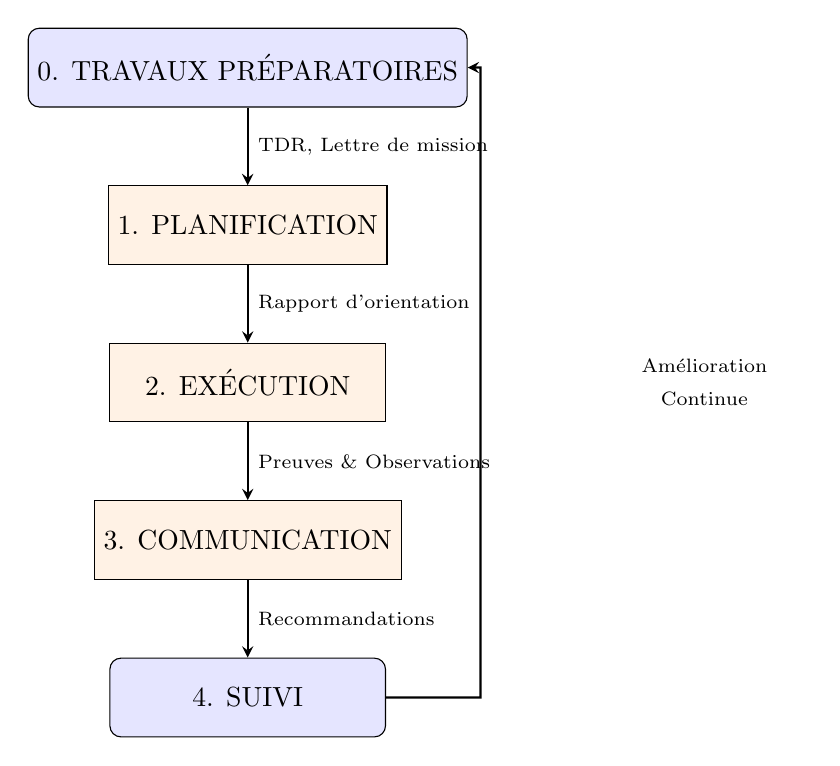
\begin{tikzpicture}[node distance=2cm]
    \tikzstyle{startstop} = [rectangle, rounded corners, minimum width=3.5cm,
        minimum height=1cm, text centered, draw=black, fill=blue!10]
    \tikzstyle{process} = [rectangle, minimum width=3.5cm, minimum height=1cm,
        text centered, draw=black, fill=orange!10]
    \tikzstyle{arrow} = [thick,->,>=stealth]

    \node (p0) [startstop] {0. TRAVAUX PRÉPARATOIRES};
    \node (p1) [process, below of=p0] {1. PLANIFICATION};
    \node (p2) [process, below of=p1] {2. EXÉCUTION};
    \node (p3) [process, below of=p2] {3. COMMUNICATION};
    \node (p4) [startstop, below of=p3] {4. SUIVI};

    \draw [arrow] (p0) -- node[anchor=west] {\scriptsize TDR, Lettre de mission} (p1);
    \draw [arrow] (p1) -- node[anchor=west] {\scriptsize Rapport d'orientation} (p2);
    \draw [arrow] (p2) -- node[anchor=west] {\scriptsize Preuves \& Observations} (p3);
    \draw [arrow] (p3) -- node[anchor=west] {\scriptsize Recommandations} (p4);

    % Boucle de feedback
    \draw [arrow] (p4.east) -- ++(1.2,0) -- ++(0,8) -- (p0.east);
    \node at (5.8,-4) [text width=2.5cm, align=center]
        {\scriptsize Amélioration Continue};
\end{tikzpicture}
\end{center}
